\documentclass[10pt]{article}

\usepackage{spheric}
%%%TITLE
\title{An elasto-plastic-$\mu$(I) SPH model for landslide induced debris flow}
\date{}

%%AFFILIATIONS

\author[1]{Wentao ZHANG$^\dagger$}
\author[1]{Yi AN}
\affil[1]{Institute of Mechanics, Chinese Academy of Sciences, P.R. China}

\author[2]{Qingquan LIU}
\affil[1]{Beijing Institute of Technology, P.R. China}
\affil[$\relax$]{\email{\dagger}{zhangwentao@imech.ac.cn}}


%%DOCUMENT
\begin{document}

\maketitle

%\SelectedTopics{}

%%PLEASE PUT YOUR ABSTRACT HERE
\begin{abstract}
 In the landslide induced debris flow problem, the soil slope experiences four stages: slope instability, large deformation, debris flow and deposition. Although the SPH method has been applied in geotechnical problems such as slope instability since Bui et al. \cite{bui2008lagrangian}, the numerical simulation of this whole process, esp. which includes phase change between solid and fluid, is very few. In this study, the elasto-plastic viscous implementation with Drucker-Prager yield criterion for solid stage and $\mu$(I) rheology for fluid stage is developed based on DualSPHysics. The yield behave of the soil is similar with Bui \cite{bui2008lagrangian} while the after yielding flow is described with $\mu$(I) rheology borrowed from granular flow. Comparing with Jutzi \& Asphaug's model \cite{jutzi2011mega} which also introduced $\mu$(I) rheology into SPH with isotropic pressure, the elasto-plastic stage is resolved more soundly in this study, especially for slope failure problems. 

The model is validated with a set of laboratory dry-granular dam break experiments with different initial aspect ratio of the reservoir. Figure \ref{fig:33} shows the shape and velocity field of the case with aspect ratio of 2.5. Good agreement is found between the simulated results and the laboratory data on both the shape evolution and the velocity field. Moreover, the simulation could also provide the shear band distribution (Figure \ref{fig:33}a) which is essential for understanding of the mechanism in this problem. Almost all parameters involved in the simulation have their physical meaning and could be obtained from experiment. Some artificial parameters focusing on numerical stability are chosen according to previous studies without tuning. This model could provide a powerful tool for the landslide induced debris flow study.

\begin{figure}[!htb]
\begin{minipage}[b]{0.5\linewidth}
\centering
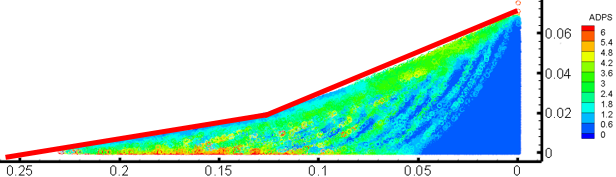
\includegraphics[width=0.9\textwidth]{33-11.png}\\ (a)

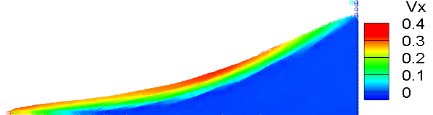
\includegraphics[width=0.9\textwidth]{33-13.png}\\ (c)
\end{minipage}
\begin{minipage}[b]{0.5\linewidth}
\centering
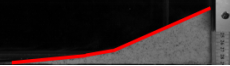
\includegraphics[width=0.9\textwidth]{33-12.png}\\ (b)

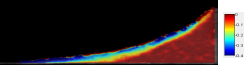
\includegraphics[width=0.9\textwidth]{33-14.png}\\ (d)
\end{minipage}
\caption{Comparison of shape and velocity between numerical and experimental results (a. simulated shape while the red solid line is final shape observed in experiment, b. observed shape, c. simulated $x$ velocity, d. $x$ velocity observed in experiment)}\label{fig:33}
\end{figure}




\end{abstract}


%%THE END OF ABSTRACT

\addbib

\end{document}
